\chapter{第二章} 
\pagenumbering{arabic} % 阿拉伯数字页码

一些例子,可以模仿。

\section{引用示例}
~20~世纪~70~年代~Crosby~和~Karnopp~提出控制算法\cite{ck1,ck2,ck3}。~1986~年,~Kim~利用~lyapunov~方法行的稳定性\cite{ck2,ck3}。同年,~Choi~等人的座椅\cite{ck3}。

\section{公式示例} 
行内公示$y_{12}$、$\dot y_{12}$、$\ddot y_1$、$\dot y_1$代入得到:
{\setlength\abovedisplayskip{3pt}
	\setlength\belowdisplayskip{3pt}
	\begin{equation}	I = \left\{ {\begin{array}{*{20}{c}}
	{{K_s}|{{\dot y}_1}|}&{,{{\dot y}_1}{{\dot y}_{12}} > 0}\\
	0&{,{{\dot x}_1}{{\dot e}_{12}} \le 0}
	\end{array}} \right.	\end{equation}}

{\setlength\abovedisplayskip{3pt}
	\setlength\belowdisplayskip{3pt}
	\begin{equation}	{K_s}(k + 1) = {K_s}(k) + \mu \left[ { - \frac{{\partial P}}{{\partial {K_s}(k)}}} \right]	\end{equation}}


\section{图片示例}
此描述如图~\ref{fig1}~所示。

\begin{figure}[!htbp]
	\centering	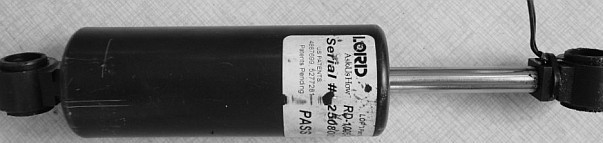
\includegraphics[width=12cm]{pic/fig1}
	\caption{长图}	\label{fig1}	\end{figure}

\begin{figure}[!htbp]
	\begin{center}
		\begin{minipage}[c]{0.44\textwidth}
			\centering		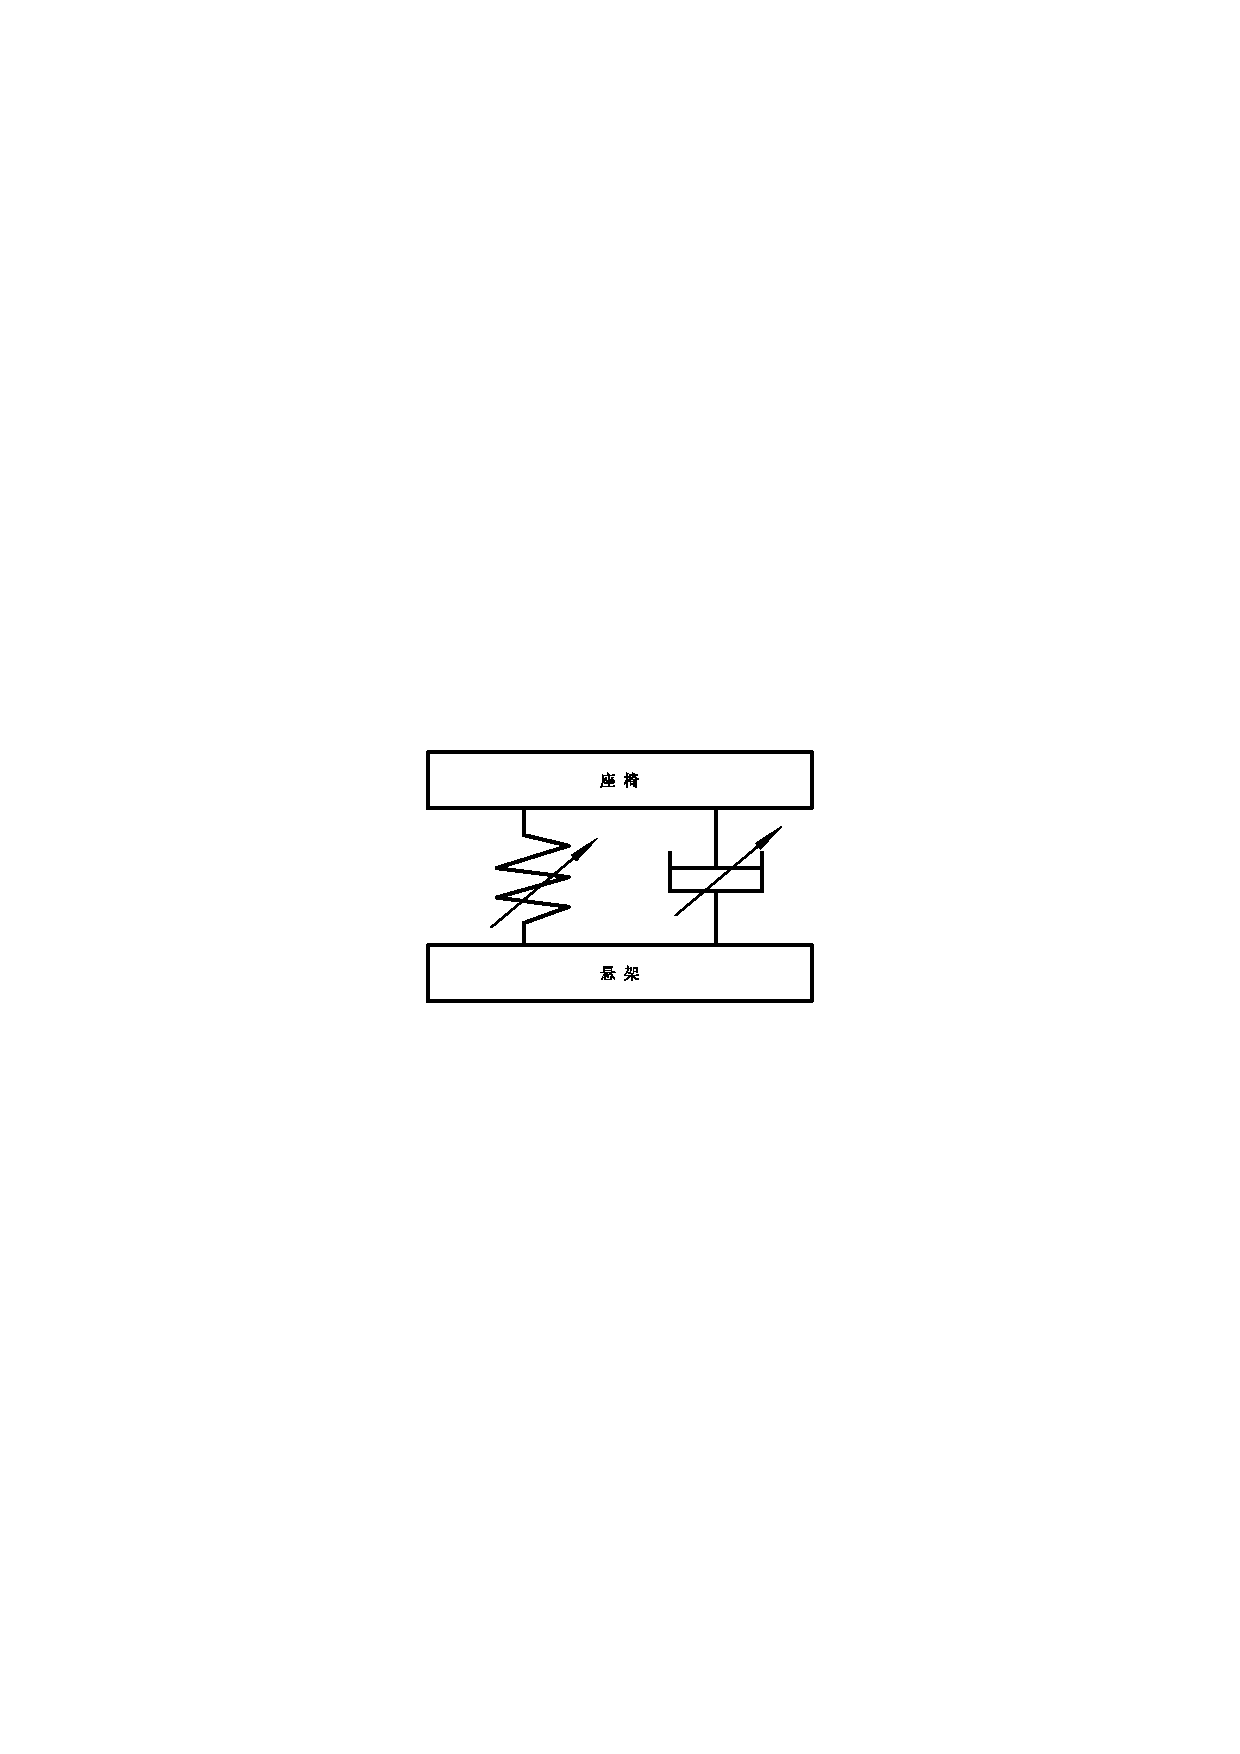
\includegraphics{pic/fig2-1}
			\caption{分图1}	\label{fig2-1}
		\end{minipage}%
		\begin{minipage}[c]{0.56\textwidth}
			\centering		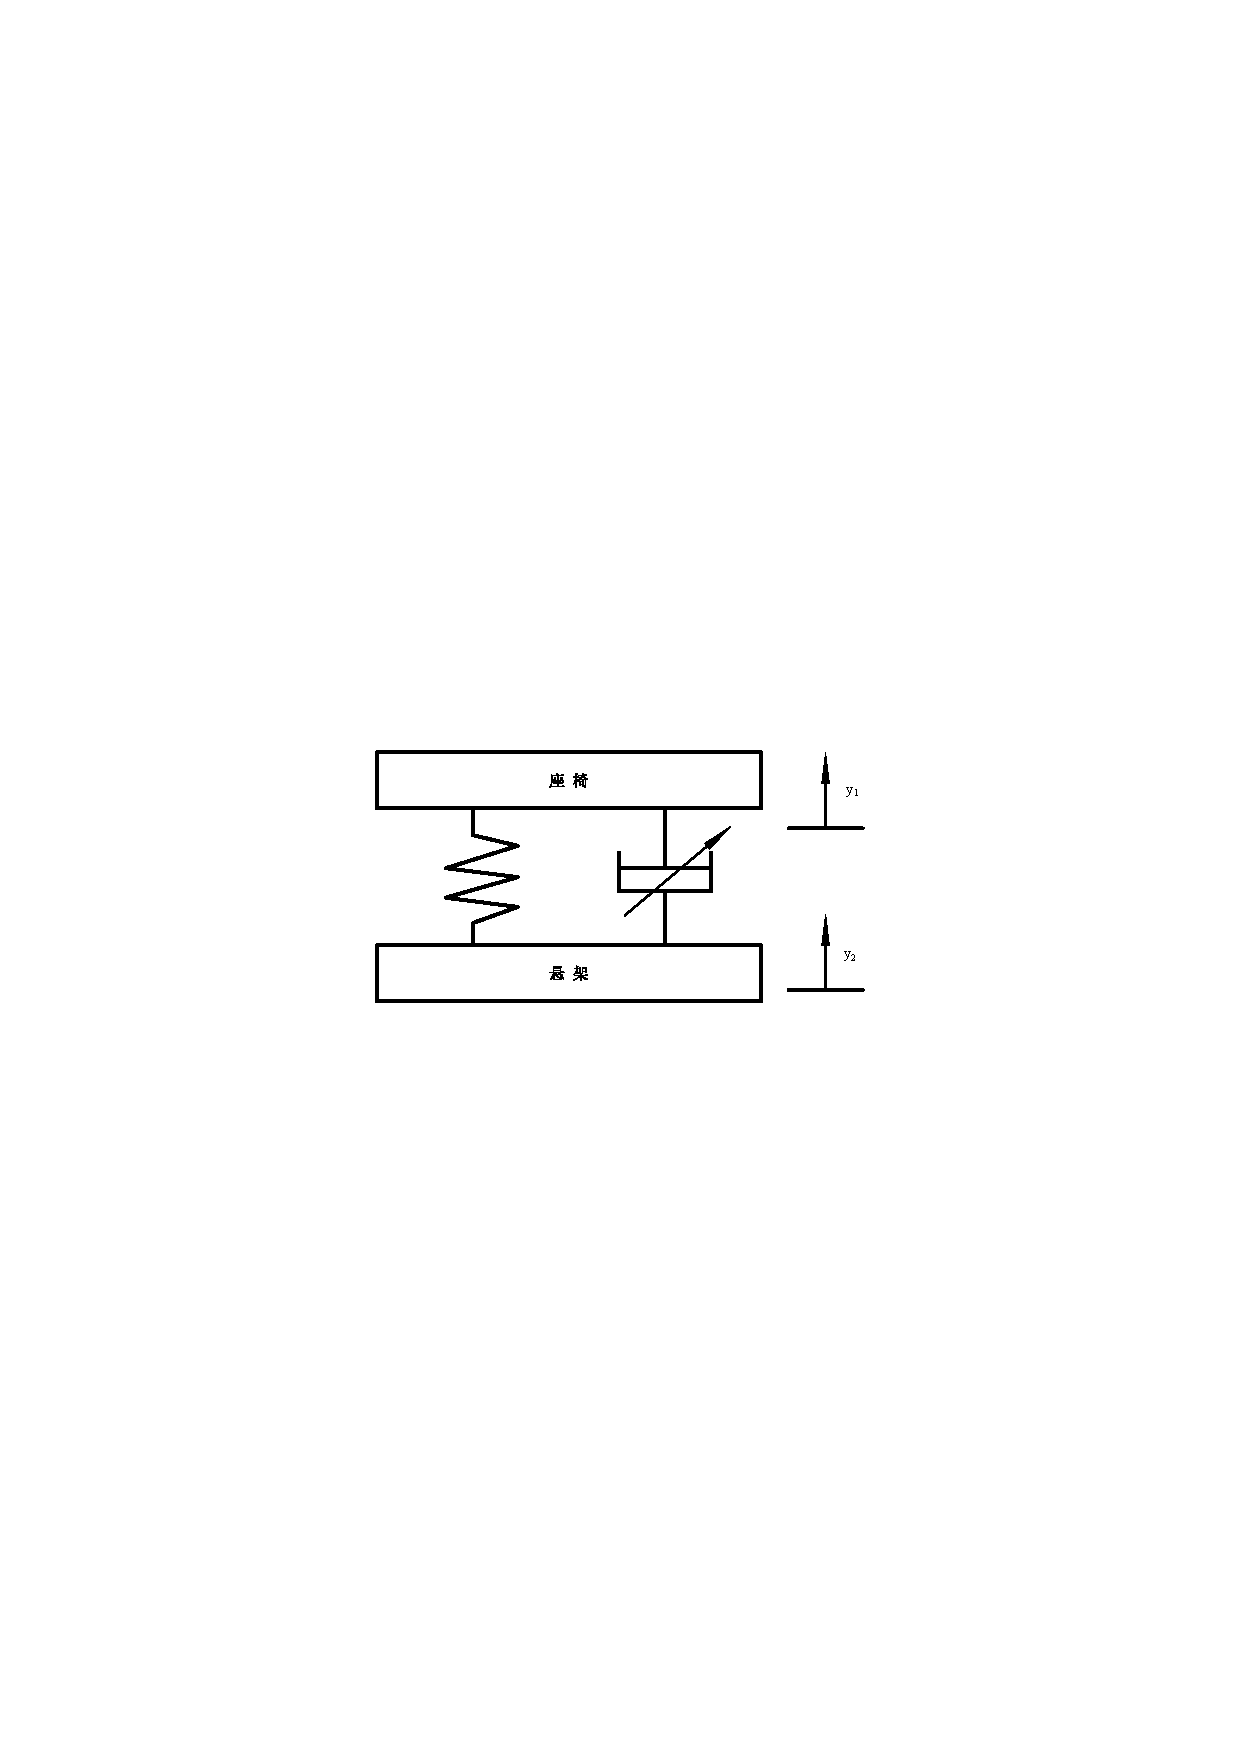
\includegraphics{pic/fig2-2}
			\caption{分图2}	\label{fig2-2}
		\end{minipage}
	\end{center}
\end{figure} 


\section{表格示例}
\begin{table}[H]
	\caption{表格示例}	\label{table1}
	\vspace{-0.5 cm} \zihao{-5}
	\begin{center}
		\begin{tabular}{cr@{.}lcr@{.}lcc}
			\toprule[1pt]
			 名  & \multicolumn{2}{c}{值} &  名  & \multicolumn{2}{c}{值} &    名     & 值 \\ \midrule[0.6pt]
			$a_0$ &  1 & 0              & $b_0$ &   2 & 73            &   $h_2$    & 0 \\
			$a_1$ &  30 & 4              & $b_1$ &   0 & 0               &   $h_3$    & 1 \\
			$a_2$ & 50 & 1              & $b_2$ &   0 & 2I+0.1          &   $h_4$    & 0 \\
			$a_3$ & -8 & 9              & $h_0$ & 111 & 1               &   $V_0$    & 0 \\
			$a_4$ & 13 & 8              & $h$ &   0 & 0               & $F_{bs}$ & 0 \\ \bottomrule[1pt]
		\end{tabular}
	\end{center}
	\vspace{-0.3 cm} \hspace{4.6 cm} {\zihao{-5} 注:此处是注释。}
\end{table}\zihao{-4} \vspace{-7pt}


\clearpage
